\documentclass[handout]{beamer}
%\documentclass[presentation]{beamer}

\usecolortheme{Imperial}
 
\usepackage[utf8]{inputenc}
\usepackage[UKenglish]{babel}
\usepackage{booktabs}
\usepackage{caption}
\usepackage{subcaption}
\usepackage{graphicx}
\usepackage{amsmath}
\usepackage{amsfonts}
\usepackage{amssymb}
\usepackage{epstopdf}

% complying UK date format, i.e. 1 January 2001
\usepackage{datetime}
\let\dateUKenglish\relax
\newdateformat{dateUKenglish}{\THEDAY~\monthname[\THEMONTH] \THEYEAR}

% Imperial College Logo, not to be changed!
\institute{\includegraphics[height=0.7cm]{/home/atarzia/presentations/imperial_beamer_template/Imperial_1_Pantone_solid.eps}}

% -----------------------------------------------------------------------------


\graphicspath{{/home/atarzia/projects/cage_collect/figures/}}
\usepackage{mhchem}
\usepackage{siunitx}
\DeclareSIUnit{\Molar}{M}
\newcommand{\btVFill}{\vskip0pt plus 1filll}
\newcommand{\footnoteline}{\noindent\rule{2cm}{0.4pt}\\}
% -----------------------------------------------------------------------------

%Information to be included in the title page:
\title{Updating the database of POCs}

%\subtitle{Subtitle}

\author{Andrew Tarzia}

\date{\today}



\begin{document}
 
\frame{\titlepage}


\begin{frame}{Search process}
\begin{itemize}
	\item Extract all REFCODEs associated with list of 23 authors using \textbf{ConQuest} OR CSD Python API
	\item Filter by:
	\begin{itemize}
		\item Has 3D coordinates
		\item Not organometallic
		\item Crystal structures only
		\item Published post 2015		
	\end{itemize}
	\item Visualize in ConQuest and keep only 'cage-like' structures
	\item Produces 108 cage structures (CDB41 has 41 structures) although this may not be exhaustive
\end{itemize}
%\centerline{\includegraphics[width=6cm]{zhu_header}}
\end{frame}

\begin{frame}{Properties of crystal structures}
\begin{itemize}
	\item Visualize all structures and determine if:
	\begin{itemize}
		\item Cage backbone is disordered
		\item Solvent is present
		\item Squeeze/Mask is used		
	\end{itemize}
\end{itemize}
\centerline{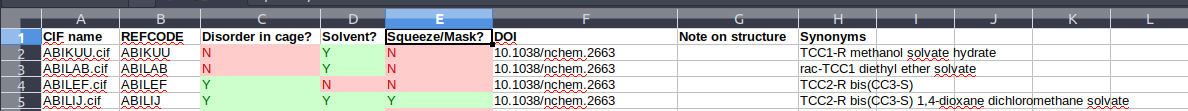
\includegraphics[width=12cm]{POC_sheet_shot}}
\end{frame}

\begin{frame}{Next steps}
\begin{itemize}
	\item Automatically clean up disorder
	\item Automatically remove solvent and extract cage molecules (pyWindow)
	\item The above process is also being applied to collect metal--organic cages from the CSD
\end{itemize}
%\centerline{\includegraphics[width=6cm]{zhu_header}}
\end{frame}



% -----------------------------------------------------------------------------
% -----------------------------------------------------------------------------
% -----------------------------------------------------------------------------

%\begin{frame}
%\frametitle{Table and Block}

%
%\begin{block}{BlockTitle}
%	something to emphasise
%\end{block}
%\end{frame}
%
%
%\begin{frame}
%\frametitle{Two Figures aside}
%\begin{columns}[b]
%\column{0.0125\textwidth}
%\column{0.4875\textwidth}
%\centering
%\begin{figure}
%	\includegraphics[draft,width=\textwidth]{fooA.pdf} \
%	% remove the 'draft' keyword, when replacing with final figure!
%	\caption{Caption of Figure A}
%\end{figure}
%\column{0.4875\textwidth}
%\centering
%\begin{figure}
%	\includegraphics[draft,width=\textwidth]{fooB.pdf} \
%	% remove the 'draft' keyword, when replacing with final figure!
%	\caption{Caption of Figure B}
%\end{figure}
%\column{0.0125\textwidth}
%\end{columns}
%\end{frame}
%
%
%\begin{frame}
%\frametitle{Text and Figure aside}
%\begin{columns}[]
%\column{0.0125\textwidth}
%\column{0.4875\textwidth}
%\centering
%\begin{figure}
%\includegraphics[draft,width=\textwidth]{fooC.pdf} \
%% remove the 'draft' keyword, when replacing with final figure!
%\caption{Caption of Figure C}
%\end{figure}
%\column{0.4875\textwidth}
%Some text and a bullet point list
%\begin{itemize}
%\item ItemA
%\item ItemB
%\item ItemC
%\item ItemD
%\end{itemize}			
%\column{0.0125\textwidth}
%\end{columns}
%\end{frame}
%
%
%\begin{frame}
%\frametitle{One Figure}
%\bigskip
%\begin{figure}
%\includegraphics[draft,width=0.8\textwidth, height=0.5\textwidth]{fooD.pdf}
%% remove the 'draft' keyword, when replacing with final figure!
%\caption{Caption of Figure D}
%\end{figure}
%\end{frame}
 
\end{document}